% vim: set ts=4 sw=4 smartindent expandtab textwidth=100:

\section{Vorbedingungen}

Gemeinsam mit unserem Betreuer haben wir uns darauf geeinigt, CrossForge zu verwenden. Die Engine unterstützt Windows, Linux und WebAssembly und benutzt nur OpenGL als Grafik API. Sie unterstützt physikalisch basiertes Rendering und Materialien, Deferred und Forward Rendering Pipelines und ein Shadersystem. Aber besonders wichtig für uns sind der Szenengraph, die Skelettanimationen und Text Rendering.

\section{Architektur und benötigte Systeme}

Aus dem MVP-Szenario und der Engine Wahl ergeben sich mehrere Anforderungen, die über verschiedene Systeme gelöst werden können. Die Roboter sind selbständige Agenten, die Entscheidungen treffen und diese auch ausführen sollen. Dieses Problem löst das Multiagentensystem. Sie müssen ihren Weg zur nächsten durstigen Pflanze finden, dafür ist das Navigationssystem zuständig. Die Roboter müssen die Pflanze gießen, was durch ein Partikelsystem visualisiert werden soll. Der Spieler und die Roboter sollen sich auf verschiedenen Plattformen bewegen und von einer zur nächsten laufen können. Zusätzlich sollen die Pflanzen verschiebbar sein. Um diese beiden Sachen zu realisieren, wird ein Physiksystem benötigt.
Der Spieler soll sich mit den Robotern unterhalten können, was durch das Dialogsystem abgedeckt wird.
Da CrossForge keinen eigenen Szenen Editor hat und die MVP Szene schon zu komplex ist, um diese mit Programmcode zu beschreiben, ist ein Szenen Editor nötig.

Um alle Systeme möglichst flexibel und unabhängig voneinander zu gestalten, haben wir uns für das Entity Component Pattern entschieden.

\section{Entity Component System}
Die klassische Herangehensweise der objektorientierten Programmierung ist der Aufbau einer Vererbungshierarchie, bei der Objekte wie der Gießroboter von allgemeingültigen Klassen abgeleitet werden. Der Roboter erbt beispielsweise, weil er sich bewegen kann, von einer Klasse Moveable und, da er gezeichnet wird, von der Klasse Renderable. Um eine Mehrfachvererbung zu verhindern, wird in der Regel eine Hierarchie eingefügt, sodass Renderable von Movable abstammt. Doch genau hier entsteht das Problem. Wenn nun ein gezeichneter Roboter erstellt werden soll, welcher sich nicht bewegen kann, so ist dies nicht mehr möglich. Grund hierfür ist die gleichzeitige Vererbung von Renderable und der Klasse Moveable. Das bedeutet, dass die Vererbungshierarchie angepasst werden muss, was bei einer großen Anzahl von Objekten und Klassen schnell sehr komplex wird. Aus diesem Grund wurde das Prinzip Entity Component Systems (ECS) eingeführt und in dem Projekt genutzt.
Das ECS besteht aus drei Bausteinen. Der erste ist die Komponente (Component), welche Informationen über Objekte hält. Im Fall des Gießroboters wären das beispielsweise Daten über dessen Position, Geschwindigkeit, Modell und noch viele mehr. Der zweite ist die Entität (Entity), welche ein Objekt in dem Projekt ist. Es besteht aus beliebig vielen Komponenten und einer ID, damit es eindeutig identifizierbar ist. Es speichert dabei keine Daten oder Programmlogik. Der letzte Teil des ECS ist das System. Es enthält die gesamte Logik, jedoch keine Daten. Ein Projekt besteht aus mehreren Systemen, die die Werte der Komponenten auslesen und anpassen. 
Beispielsweise liest ein SteeringSystem die Geschwindigkeit aus einer SteeringComponent und aktualisiert basierend darauf die Position in der Positionskomponente. Der große Vorteil besteht darin, dass die Eigenschaften eines Objekts leicht angepasst werden können, indem die Werte seiner Komponenten ändert, oder sogar ganze Komponenten hinzufügt beziehungsweise entfernt werden.
\section{Partikelsystem}
Partikelsysteme werden verwendet, um natürliche Phänomene, wie Wasser, Rauch oder Feuer darzustellen. Dabei gibt es stets einen sogenannten Emitter, welcher Partikel ausstößt. Diese besitzen einige Eigenschaften, wie beispielsweise Lebensdauer, Position und Richtung. Damit sie sichtbar werden, müssen ihnen grafische Merkmale, wie ein Modell, Textur und Material, zugeordnet werden. Durch die grafische Beschaffenheit, die Anzahl der Partikel und ihr Verhalten untereinander können verschiedene natürliche Phänomene simuliert und dargestellt werden. In dem Projekt wird das Partikelsystem verwendet, um dem Nutzer ein visuelles Feedback zu geben, wenn ein Roboter eine Pflanze gießt. In diesem Fall wird ein Wasserstrahl, wie er von einer Gießkanne erzeugt wird, simuliert.

\section{Multiagentensystem}

Das Multiagentensystem ist das Herz unseres Projektes, da das Verhalten von allen belebten und unbelebten Agenten von diesem System gesteuert werden soll. Man unterscheidet zwischen Zentraler KI und Agentenbasierter KI. Bei Zentraler KI werden die Entitäten von einem externen, globalen und allwissenden System gesteuert. Individuen haben deswegen keine Kontrolle über ihre eigenen Handlungen. Zentrale KI wird sehr oft eingesetzt, weil sich damit Gruppendynamiken und taktische Vorgehensweisen einfacher implementieren lassen. Bei Agentenbasierter KI treffen die Agenten unabhängige und individuelle Entscheidungen basierend auf den Informationen, die ihnen bereit stehen. Es gibt zwar trotzdem globale Informationen, die aber nicht dafür missbraucht werden dürfen, die Handlungen eines Agenten zu diktieren. Wir haben uns für Agentenbasierte KI entschieden, weil sie für unser Szenario leichter umzusetzen ist. Die Hoffnung ist, dass die Akteure dadurch natürliche Verhaltensweisen und Interaktionen zur Schau stellen.

In verschiedenen GDC \cite{YouTube_2019}\cite{YouTube_2022}\cite{YouTube_2023} Talks wurde empfohlen, ein KI-Systen in mehreren Schichten aufzubauen:

\begin{itemize}
\item Sensoren
\item Entscheidungsfindung
\item Entscheidungsausführung
\item Bewegungssteuerung
\end{itemize}

\subsection{Sensoren}

Sensoren sind ein Querschnittskonzept und tauchen deshalb in allen Ebenen auf. Sie filtern Informationen aus der Umgebung und stellen diese der Schicht bereit, in der sie eingesetzt werden. Zusätzlich können Informationen über Blackboards mit anderen Agenten geteilt werden.

\subsection{Entscheidungsfindung}

Für die Entscheidungsfindung standen die folgenden Algorithmen in der näheren Auswahl: Beliefs, Desires, Intentions (BDI), Goal Oriented Action Planning (GOAP) und Finite State Machines (FSM). Am Ende haben wir uns für Finite State Machines entschieden, weil das das einfachste Verfahren war und vorerst für die Roboter ausreicht.

Eine State Machine ist ein gerichteter Graph mit limitierter Anzahl an Stati und Aktionen. Der Agent wechselt von einem Status in den nächsten, falls eine Bedingung erfüllt ist. In unserer Simulation sollen FSMs für die Roboter eingesetzt werden, um die Stati \textit{Pflanzen gießen}, \textit{Dialog mit Spieler}, \textit{Spieler folgen}, etc. abdecken zu können. 

\subsection{Entscheidungsausführung}

Wenn der Agent eine Entscheidung getroffen hat, dann lässt sich diese Entscheidung meistens in weitere Teilprozesse zerlegen. Wenn ein Roboter zum Beispiel entschieden hat, dass er jetzt Pflanzen gießt, dann muss er:

\begin{itemize}
\item eine durstige Pflanze finden
\item zur Pflanze hinfahren
\item die Gießkanne zur Pflanze ausrichten
\item und schließlich die Pflanze gießen
\end{itemize}

Diese Sequenz von Handlungen lässt sich nur sehr schlecht mit FSMs darstellen, weswegen dieser Nachteil durch Behaviour Trees ausgeglichen werden soll. Behaviour Trees sind sehr gut darin, solche Sequenzen darzustellen oder sogar nebenläufige Handlungen zu beschreiben. Ihr Nachteil ist jedoch, dass sie nur sehr schwierig auf Übergänge von einen Status in den nächsten reagieren können. Ein Beispiel hierfür ist, dass der Spieler den Roboter anspricht und ihn über Pflanzen befragt. Um das mit Behaviour Trees festzustellen, müssen überall Monitore eingebaut werden, die dieses Ereignis erkennen und behandeln. Das macht den Baum unübersichtlich und nicht wartbar. Behaviour Trees und State Machines ergänzen sich also sehr gut.

In Behaviour Trees werden Handlungen durch Knoten beschrieben. Die Knoten können die Stati \textit{Laufend}, \textit{Fehler} oder \textit{Abgeschlossen} haben.
Knoten können dabei über die Bearbeitung ihrer Kindknoten entscheiden. Bei einem Sequenzknoten werden die Kinder von links nach rechts abgearbeitet. Nur wenn der Knoten den Status \textit{Abgeschlossen} hat, wird der rechte Geschwisterknoten aufgerufen. Wenn der Status \textit{Laufend} ist, dann wird der Knoten solange bearbeitet, bis der Status \textit{Abgeschlossen} oder \textit{Fehler} erreicht ist. Bei dem Status \textit{Fehler} wird die Abarbeitung abgebrochen und dieser nach oben propagiert. Der Elternknoten kann dann entscheiden, wie dieser Fehlerstatus behandelt wird.
Der Fallbackknoten behandelt den Fehler zum Beispiel, indem er den ersten Kindknoten findet, der nicht fehlschlägt und somit erfolgreich ausführt. Nur wenn alle Kindknoten fehlschlagen, ist der Status des Fallbackknotens \textit{Fehler}.

\subsection{Bewegungssteuerung}

Die Ebene der Bewegungssteuerung ist dafür verantwortlich, die Entscheidungen in Beschleunigung, Geschwindigkeit und Rotation umzuwandeln. Dafür haben wir uns Steering Behaviour \cite{SteeringBehaviour} näher angeschaut. Es gibt verschiedene Bewegungsmuster:

\begin{itemize}
\item Seek
\item Wander
\item Collision Avoidance
\item Queue
\item ...
\end{itemize}

Für uns ist vor allem Collision Avoidance in Verbindung mit Seek interessant.
\begin{figure}[h]
	\centering
	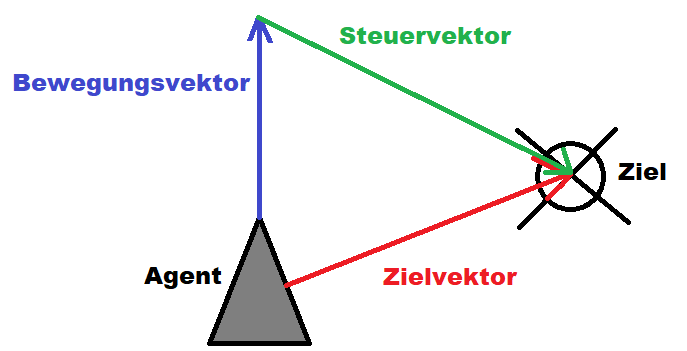
\includegraphics[height=0.3\pageheight,keepaspectratio]{pics/Seeking} 
	\caption{Suchverhalten des Roboters}
\end{figure}
Das Suchverhalten(Seek), bedeutet, dass der Agent sich auf einen Zielpunkt zubewegt und sich dabei in die richtige Richtung dreht. Dies geschieht mit Hilfe von Vektoren.
Zum einen wird ein Zielvektor genutzt, dieser zeigt von der Position des Roboters in Richtung des Ziels. Des Weiteren gibt es einen Bewegungsvektor, welcher in die Richtung zeigt, in die der Agent sich aktuell bewegt und schaut. Die Länge des Vektors entspricht dabei seiner aktuellen Geschwindigkeit. 
Um nun dessen Fahrtrichtung anzupassen, wird ein Steuervektor benötigt, der aus der Subtraktion des normierten Zielvektors und des Bewegungsvektors entsteht. Jetzt kann der Bewegungsvektor angepasst werden, sodass er in die richtige Richtung zeigt. Dazu werden der Steuervektor und Bewegungsvektor addiert. Das Problem hierbei ist, dass bei dieser Umsetzung der Roboter sofort in Richtung des Ziels schaut und sich auf dieses zubewegt. Dieses Verhalten ist unrealistisch. Aus diesem Grund erhält der Roboter zusätzliche Eigenschaften, wie Masse, maximale Geschwindigkeit und Lenkkraft. Beim Addieren der beiden Vektoren, wird der Lenkvektor zuerst durch die Masse geteilt, dadurch wird die Länge des Vektors reduziert und der Effekt verringert. Zudem muss sichergestellt werden, dass der Betrag des Vektors kleiner gleich der maximalen Lenkkraft ist. Ebenso darf der Bewegungsvektor nicht größer sein als die Höchstgeschwindigkeit. Wenn diese Anforderungen berücksichtigt werden, dreht sich der Roboter pro Schleifendurchlauf nur um einen kleinen Anteil und fährt ein Stück in Richtung Ziel. Dieses Verhalten wirkt für einen Betrachter realistischer. 
\begin{figure}[h]
	\centering
	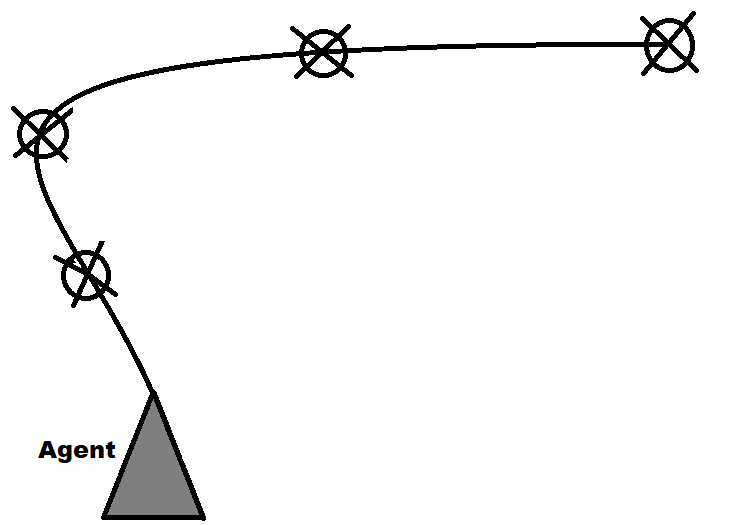
\includegraphics[height=0.3\pageheight,keepaspectratio]{pics/Pathfollowing} 
	\caption{Pfadverfolgen durch angepasstes Suchverhalten}
\end{figure}
Das zweite Lenkverhalten, das in dem Projekt genutzt wurde, ist das Verfolgen eines Pfades. Dazu wird das Suchverhalten so angepasst, dass der Roboter zahlreiche Zielpunkte entlang des Pfades sucht. Er ist zu dem Zeitpunkt jedoch noch nicht in der Lage, zu wissen, wann er an einem Ziel ankommt. Dazu wird eine weitere Funktion und der Vektor zwischen Agenten und Zielposition benötigt. Der Roboter ist angekommen, wenn die Länge des Zielvektors kürzer ist als der Radius des Agenten plus einen Sicherheitsabstand. Währenddessen muss sichergestellt werden, dass der Roboter nicht mit Hindernissen, Robotern oder Spielern kollidiert. 
\begin{figure}[h]
	\centering
	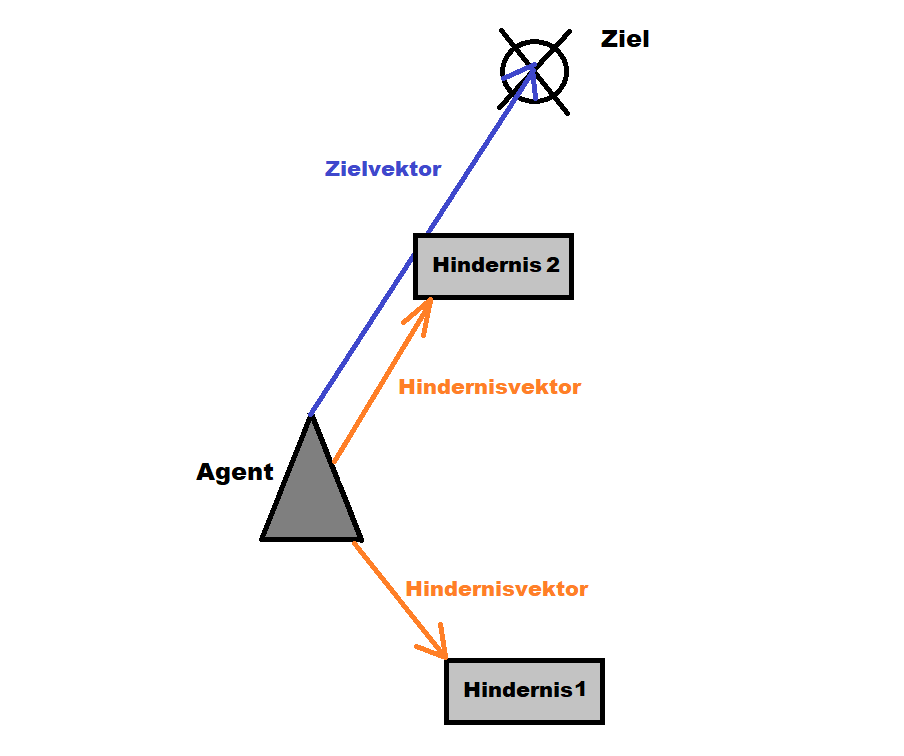
\includegraphics[height=0.3\pageheight,keepaspectratio]{pics/Avoidance1} 
	\caption{Testen der Hindernisse auf ihre Position in Relation zum Zielpunkt und der Position des Roboters}
\end{figure}
Dazu wird eine Liste aller möglichen Hindernisse auf ihre Distanz zum Agenten überprüft und geordnet. Nun wird getestet, ob sich das Hindernis zwischen Roboter und Ziel befindet, oder hinter dem Agenten. Hierfür wird das Kreuzprodukt aus dem Zielvektor und dem Vektor, der vom Roboter ausgehend in Richtung Hindernis zeigt, gebildet. Nur wenn dieses kleiner als Null ist, befindet sich das Hindernis vor dem Agenten und muss weiter getestet werden. 
\begin{figure}[h]
	\centering
	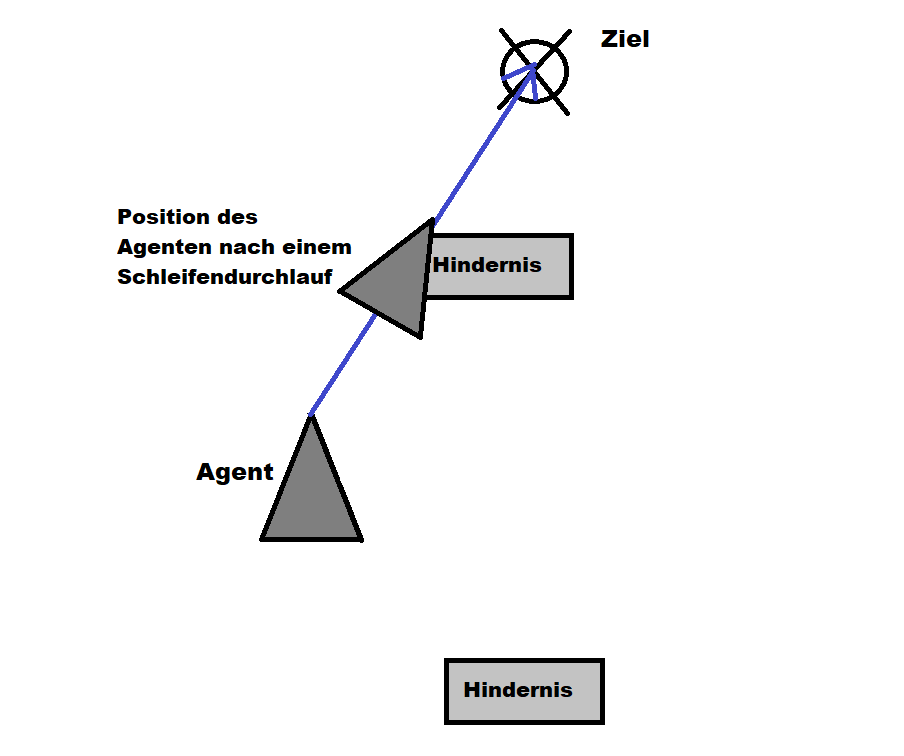
\includegraphics[height=0.3\pageheight,keepaspectratio]{pics/Avoidance2} 
	\caption{Testen auf mögliche Kolission nach einem Schleifendurchlauf}
\end{figure}
Im nächsten Schritt wird die Position bestimmt, an der sich der Roboter in dem nächsten Schleifendurchlauf befinden wird. An dieser Stelle wird der Abstand zwischen ihm und dem Hindernis betrachtet. Solange dieser nicht kleiner ist als der Roboterradius plus einen Sicherheitsabstand plus den Hindernisradius kann davon ausgegangen werden, dass der Roboter mit diesem nicht kollidieren wird. Ist der Abstand jedoch kleiner, so muss der aktuelle Wegpunkt so angepasst werden, dass der Roboter dem Hindernis ausweicht. 
\begin{figure}[h]
	\centering
	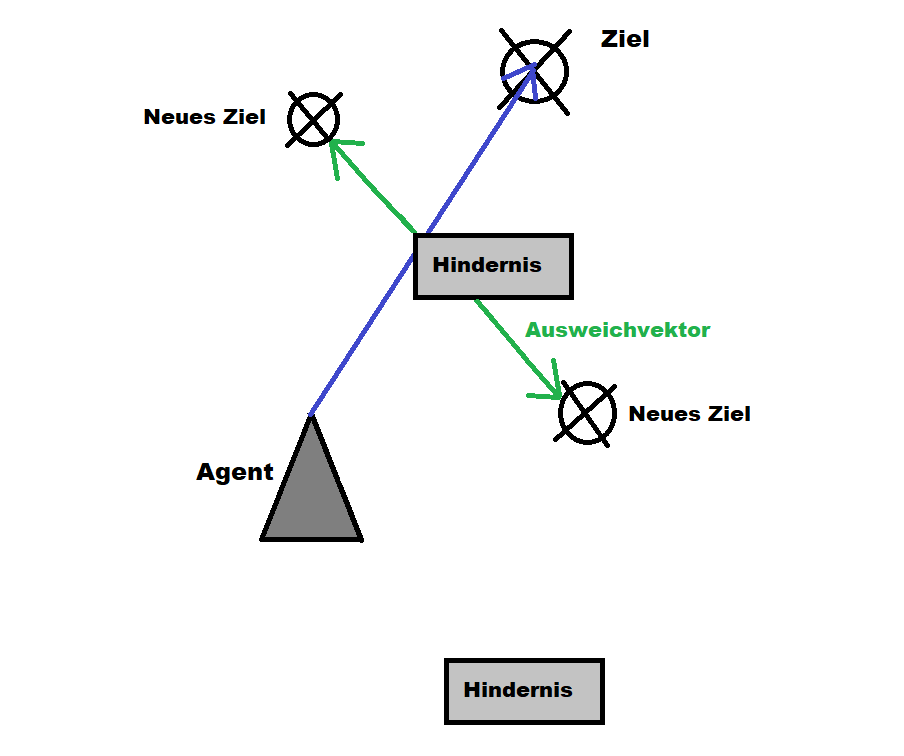
\includegraphics[height=0.3\pageheight,keepaspectratio]{pics/Avoidance3} 
	\caption{Verschieben des Zielpunktes}
\end{figure}
Dies geschieht, indem ein Vektor erzeugt wird, der von dem Hindernis weg zeigt. Es werden nun zwei potenzielle neue Wegpunkte erzeugt, die sich rechts beziehungsweise links von dem Hindernis befinden. Nun wird überprüft, bei welchem der beiden die Abweichung vom aktuellen Pfad kleiner ist. Dieser wird als der neue Wegpunkt gesetzt und der alte wird entfernt. Der Roboter bewegt sich nun auf diesen zu und weicht dem Hindernis aus.
\begin{figure}[h]
	\centering
	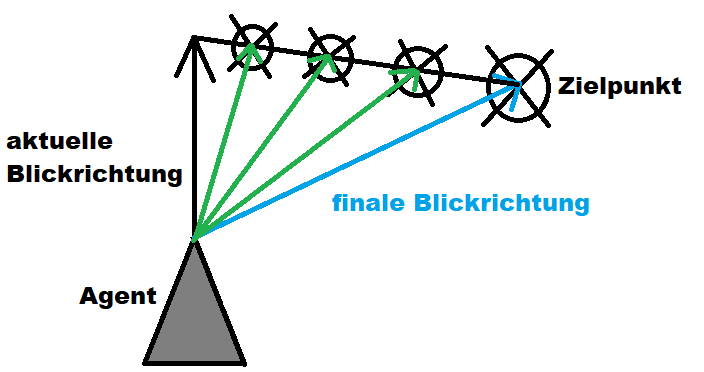
\includegraphics[height=0.3\pageheight,keepaspectratio]{pics/TurnTo} 
	\caption{Drehen des Roboters}
\end{figure}
Das letzte Lenkverhalten ist das auf der Stelle Drehen. Dieses wird genutzt, wenn der Spieler mit dem Roboter redet oder er eine Pflanze gießen will. Um die Verhaltensweise umzusetzen, werden die Zielrichtungen benötigt, in die der Agent final schauen soll und seine aktuelle Blickrichtung. Er soll sich dabei wieder nur langsam drehen, um ein realistisches Verhalten zu simulieren. Mit Hilfe von linearer Interpolation werden zusätzliche Punkte zwischen der Ausgangssituation und der Zielrichtung gebildet. Der Roboter kann sich nun nach und nach in Richtung dieser ausrichten. Das hat zur Folge, dass er sich nur langsam dreht. Durch das Berechnen der einzelnen Zwischenpunkte ist diese Umsetzung zusätzlich unabhängig von der Framerate.

\section{Navigationssystem}

In der Mitte der MVP-Szene befindet sich die Wendeltreppe, weswegen die Roboter nicht immer den direkten Weg zur Pflanze fahren können, weil sie dieses Hindernis beachten müssen. Das Navigationssystem übernimmt die Aufgabe, einen Pfad von einem Startpunkt zum Zielpunkt zu finden. Um Zeit zu sparen und uns auf die Hauptaufgabe konzentrieren zu können, haben wir uns entschieden, die Bibliothek Recast und Detour einzusetzen. Recast berechnet das Navigationsmesh aus der statischen Geometrie, und Detour findet zur Laufzeit einen Pfad auf diesem Navigationsmesh. Da das Navigationsmesh nicht dynamisch angepasst werden muss, reicht es aus, wenn man es einmal vor der Kompilierung berechnet, speichert und dann in CrossForge lädt. Die Bibliothek stellt hierfür ein Beispielprogramm bereit, was wir nutzen.

\section{Physiksystem}

Die Entities und der Spieler sollen mit der statischen Szenengeometrie und sich selber kollidieren. Um diese Kollisionen zu erkennen und aufzulösen, ist das Physiksystem nötig. Dafür möchten wir die Bullet Bibliothek einsetzen, da Linus schon einmal den Separating Axis Theorem Algorihmus in 2D implementiert hat und das sich als sehr zeitaufwändig und fehleranfällig herausgestellt hat. 


\section{Szenen Editor}

Wir benötigen einen Szenen Editor, weil schon bei einer geringen Anzahl an platzierten Entitäten der Code unübersichtlich und schwer zu warten ist. Als Alternative könnten wir die Agenten und Pflanzen prozedural platzieren, was aber ein zu komplexes Gebiet wäre und damit den Rahmen sprengen würde. Selber einen Szenen Editor von Grund auf neu zu schreiben ist keine Option, weil auch das eine riesige Aufgabe ist. Deswegen haben wir uns dazu entschieden, die Open Source Software Blender zu verwenden. Blender ist ein mächtiger 3D-Editor, den man über Addons erweitern kann. Somit haben wir zwei Möglichkeiten, unsere Szenen zu erstellen und in CrossForge zu laden. Wir können die Szene als GLTF-Datei exportieren und dann die vorhandenen Funktionen in CrossForge erweitern, um aus der GLTF-Datei die einzelnen Transformationen für die Entitäten zu extrahieren. Oder wir schreiben ein Add-On, welches die Szene nach unseren Anforderungen exportiert.

\subsection{GLTF als Szenenbeschreibung}

Khronos Group veröffentlichte am 19.10.2015 das offene GLTF Format, um dreidimensionale Szenen und Modelle darzustellen. In dem Format können Szenen mit ihren Knoten, Kamerainformationen, Animationen, Texturen, Materialien und natürlich auch Modellinformationen gespeichert werden. CrossForge unterstützt über die Assimp Bibliothek verschiedene Dateiformate, unter anderem auch GLTF.

Die Idee ist, dass alle Entities einer bestimmten Namenskonvention folgen. Die Szene wird als Ganzes in das GLTF-Format exportiert und mit Assimp geladen. Assimp hat einen eigenen Szenengraph, den man traversieren kann, und wenn man an einem Knoten mit bestimmter Namenskonvention angelangt ist, weiß man, dass es sich um ein Entity handelt. Die Transformation des Knotens wird dann zur Transformation des Entities. Alle Kindknoten können dann zu einem Modell zusammengefasst werden und für die Geometriekomponente des Entities benutzt werden.

Dieser Ansatz hat den Vorteil, dass er editoragnostisch ist, und wir können vorhandenes Wissen über Assimp nutzen. Leider hat diese Variante aber auch große Nachteile: man muss die Änderungen ziemlich tief in CrossForge vornehmen, was sehr viele Code-Änderungen nach sich zieht. Der Szenenersteller muss die Knoten im Editor korrekt benennen, weil man sie in CrossForge sonst nicht mehr erkennen kann.

\subsection{Eigenes Format zur Szenenbeschreibung}

Wir können ein Blender Plugin schreiben, das die Transformationen der einzelnen Entities in eine JSON-Datei exportiert. Das Problem ist, dass Blender erkennen muss, was statische Geometrie ist und was Entities sind. Es gibt aber eine Funktion, um externe .blend-Dateien in die aktuelle Szene zu linken. Jetzt kann man die Regel aufstellen, dass alles, was gelinkt ist, ein eigenes Entity ist. Die Vorteile sind, dass keine Eingriffe ins Engine-Innere nötig sind und auch die Implementierung auf CrossForge-Seite sehr simpel ist, da man das Dateiformat selber bestimmen kann. Der Nachteil ist, dass noch niemand von uns ein Blender Add-On geschrieben hat und wir deswegen noch keine Erfahrung in diesem Bereich haben.

\section{Dialogsystem}

Wir haben uns dazu entschieden ein Dialogsystem zu implementieren, damit man als Nutzer mit den Robotern kommunizieren kann. Der Nutzer soll dazu ein Dialogfenster öffnen können, wenn er sich nah genug an einem Roboter befindet. Im Dialogfenster werden dann die Aussagen des Roboters und die Antwortoptionen des Nutzers angezeigt. Durch Klicken auf die Antworten wird der Dialog fortgesetzt. Wenn der Dialog beendet ist wird das Dialogfenster wieder geschlossen. Ziel des Dialogsystems für das Minimum Viable Product ist es, dass man den Roboter nach dem Name einer Pflanze fragen kann. 

\subsection{Imgui}

Unsere erste Idee für die Umsetzung des Dialogfensters war die Features zu nutzen, die in CrossForge schon implementiert waren. Dafür wollten wir ursprünglich Texturen verwenden. Da das allerdings wahrscheinlich sehr aufwendig geworden wäre, hat Linus vorgeschlagen Imgui zu nutzen.
Imgui ist eine C++-Bibliothek für grafische Benutzeroberflächen. Normalerweise ist Imgui zwar eher für Debug-Tools gedacht, da es grafisch relativ simpel ist und nur sehr eingeschränkte Möglichkeiten zur grafischen Individualisierung bietet. Für unsere Zwecke ist es aber trotzdem gut geeignet, weil es uns, insbesondere für das Minimum Viable Product, wichtiger ist schnell ein Dialogfenster angezeigt zu bekommen als, dass es besonders hübsch aussieht. 

\subsection{JsonCpp}

Die Dialoge selbst wollen wir in Json-Dateien speichern. Json-Dateien ermöglichen es uns zum einen die Dialoge vom Code zu trennen und somit zum anderen leicht neue Dialoge hinzuzufügen und andere Dialoge auszuwählen. Damit wir die Daten aus diesen Dateien auslesen können nutzen wir JsonCpp, eine C++-Bibliothek, die es ermöglicht Json-Dateien mit C++ ein- und auszulesen. 

\subsection{Dialoggraph}

Als Datenstruktur für den Dialog nutzen wir eine Baumstruktur. Dabei beinhaltet jeder Knoten einen Text, einen Boolean, der angibt ob der Text vom Spieler gesprochen wird, und eine Liste mit möglichen Antworten, die jeweils durch weitere Knoten repräsentiert werden. Dieser Baum wird erstellt, indem die entsprechenden Informationen aus einer Json-Datei ausgelesen werden. 

\subsection{Dialogmap}

Um den Dialog zum Erfragen eines Pflanzennamens umsetzen zu können, benötigt man im Dialog in der Json-Datei einen Platzhalter für den Name der Pflanze. Dieser Platzhalter wird dann durch den entsprechenden Name ersetzt. Dafür wollen wir eine Map nutzen, die den Platzhalter als Key entgegen nimmt und einen Funktionspointer zurückgibt. Mithilfe der dadurch aufgerufenen Funktion wird dann der Name der Pflanze in Abhängigkeit von der Position des Roboters und der Position des Spielers ermittelt, sodass die Map letztendlich indirekt den Pflanzennamen zurückgibt.  
\par
Die Nutzung einer Map ermöglicht es schnell und einfach neue Platzhalter/Keys hinzuzufügen, durch die auch andere Ersetzungen mithilfe entsprechender Funktionen möglich sind. Die genutzten Funktionen können aber auch andere Funktionalitäten erfüllen als nur einfache Textersetzungen; eine Funktion kann auch beispielsweise ein Event auslösen. Ein solches Event könnte zum Beispiel sein, dass man den Roboter anweist dem Spieler zu folgen oder aus dem Weg zu gehen.

\section{Modelle und Szene}

Die Szene und die zugehörigen Modelle sind von wesentlicher Bedeutung, um alle anderen Funktionen überhaupt darstellen zu können. Natürlich könnte man dafür auch jedes beliebige Modell verwenden, sogar einen simplen Würfel. Dennoch hatten wir ein klares Bild davon, was wir darstellen möchten. Wie bereits im Abschnitt Motivation erläutert, besteht unser MVP aus zwei Plattformen, jeweils einem Roboter und mehreren Pflanzen.
\par
Der erste und entscheidendste Schritt war, zu überlegen, wie unsere Roboter aussehen sollten, da sie die Hauptakteure in unserem Projekt sind und direkt mit dem Spieler interagieren. Ursprünglich war geplant, den Robotern ein eher menschenähnliches Design zu verleihen. Allerdings entschieden wir uns zunächst für eine simplere Gestaltung. Daher habe ich mich für ein eher "simples und knuffiges" Design entschieden und verschiedene Konzepte skizziert. Zusätzlich habe ich mir Gedanken über potenzielle Funktionen gemacht und diese als Randnotizen zum Design festgehalten.
\begin{figure}[h]
	\centering
	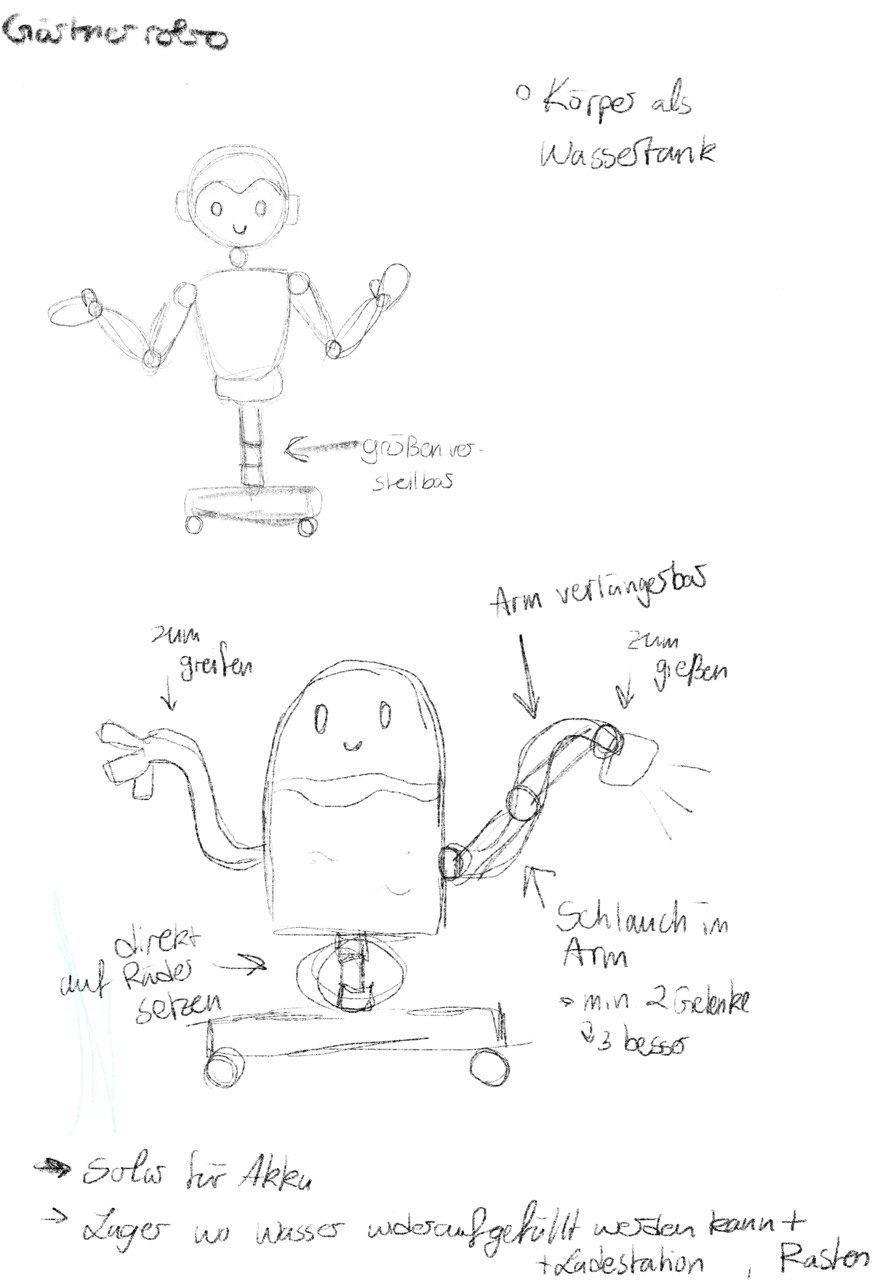
\includegraphics[height=0.3\pageheight,keepaspectratio]{pics/1} 
	\caption{Konzeptskizze für den Roboter}
\end{figure}
\par
Eine weitere Überlegung war, den Roboter schweben zu lassen anstatt ihn zu fahren, um zusätzliche Programmierungsaufwände zu vermeiden. Jedoch wurde diese Idee zunächst als zu futuristisch angesehen und daher vorerst abgelehnt. Bei der abschließenden Skizzierung habe ich das Radsystem erneut überdacht und im Nachhinein noch einige Änderungen vorgenommen.
\begin{figure}[H]
	\centering
	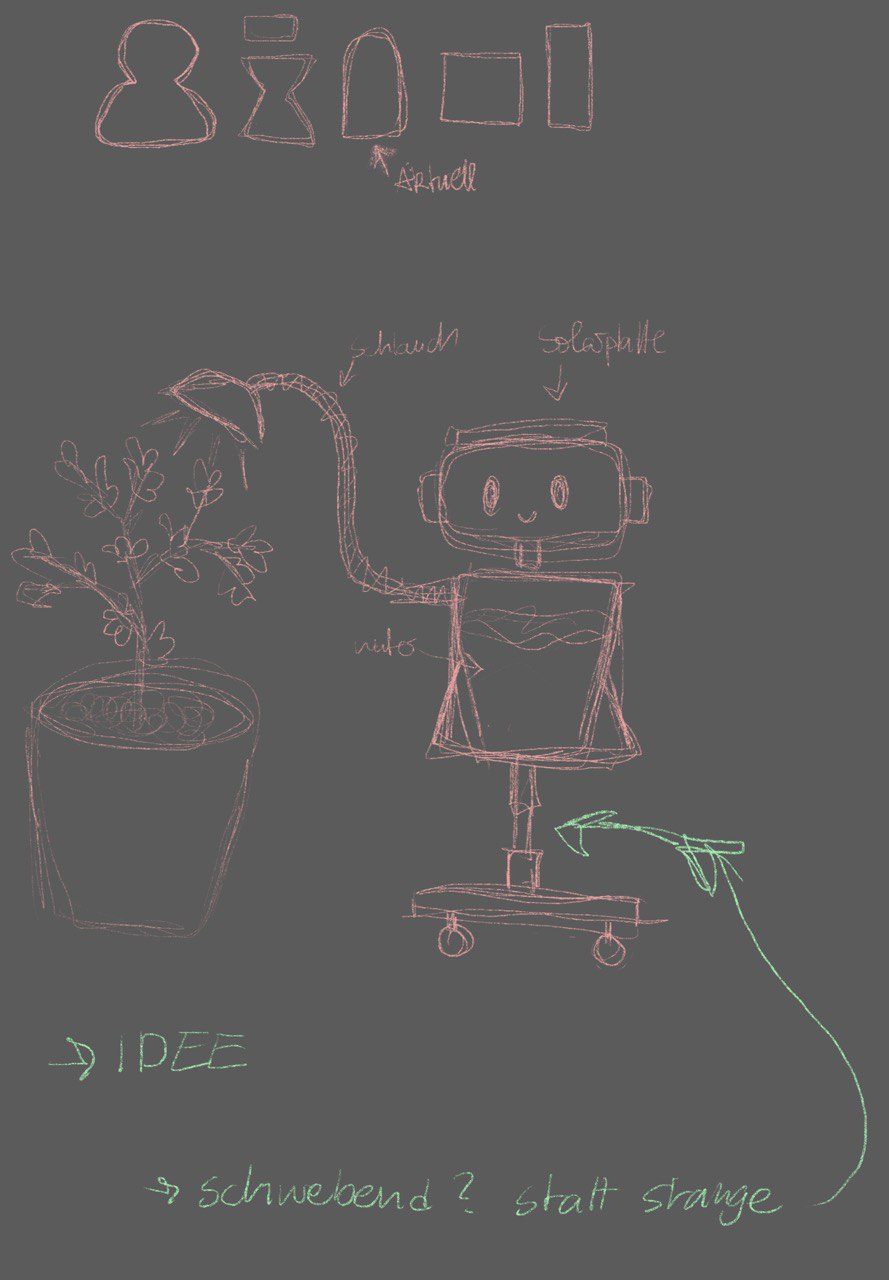
\includegraphics[height=0.2\pageheight,keepaspectratio]{pics/2} 
	\caption{Finaler Entwurf für den Gärtnerroboter}
\end{figure}
\par
Die nächsten Überlegungen galten den Pflanzen. Dabei habe ich eher spontan gearbeitet, ohne vorherige Skizzen. Es war mein Ziel, eine einfache und eine eher exotische Pflanze zu gestalten, um etwas Variation zu erreichen.
\par
Die Gestaltung der Plattformen und der Szene im Allgemeinen erforderte ähnlich viel Aufwand wie bei den Robotern im Konzept. Auch hier habe ich zahlreiche Ideen skizziert und im Anschluss diskutiert. Anfangs habe ich weitreichend gedacht und komplexere Szenen entworfen.
\begin{figure}[H]
	\begin{subfigure}{0.5\textwidth}
		\centering
		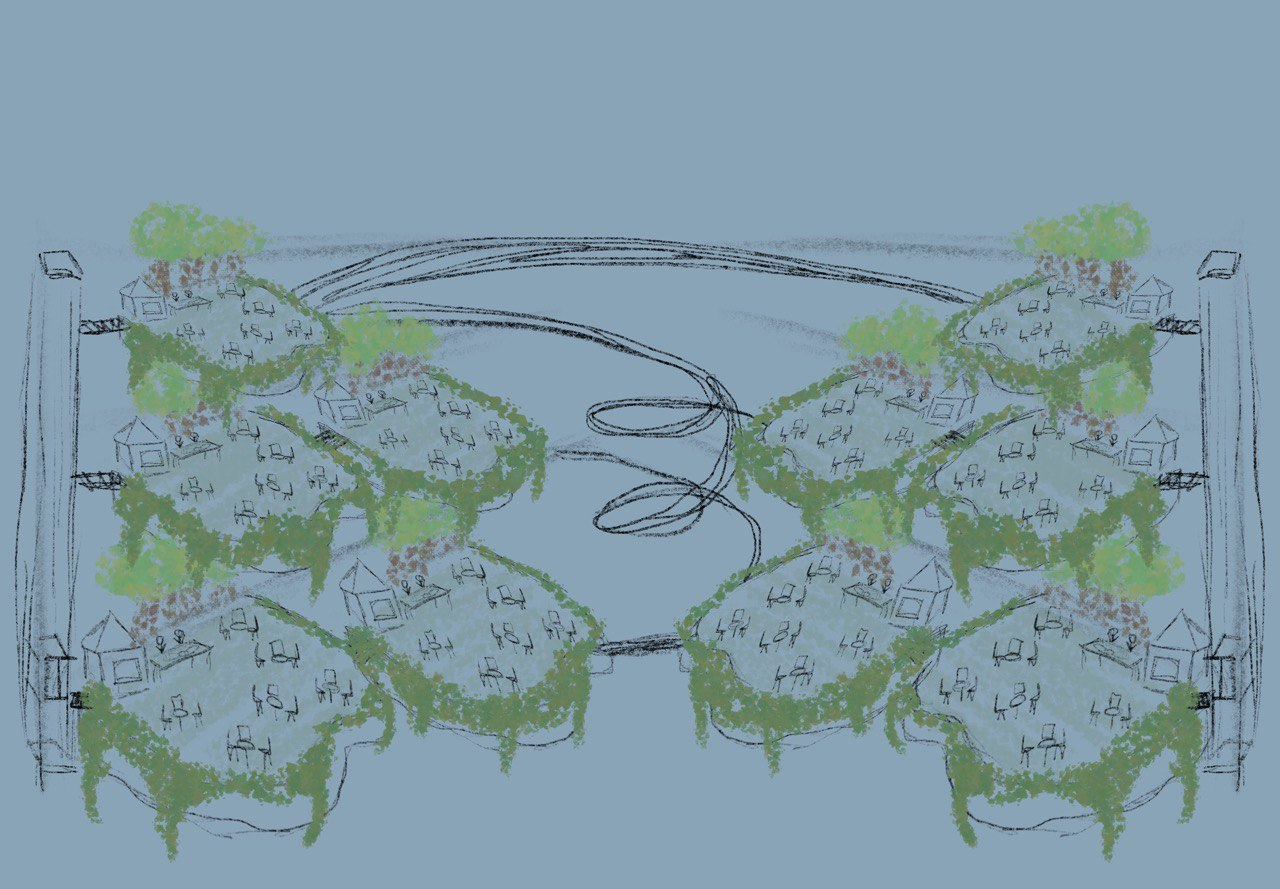
\includegraphics[height=0.3\pageheight,keepaspectratio]{pics/3} 
		\caption{Ursprüngliche Idee}
	\end{subfigure}	
	\begin{subfigure}{0.5\textwidth}
		\centering
		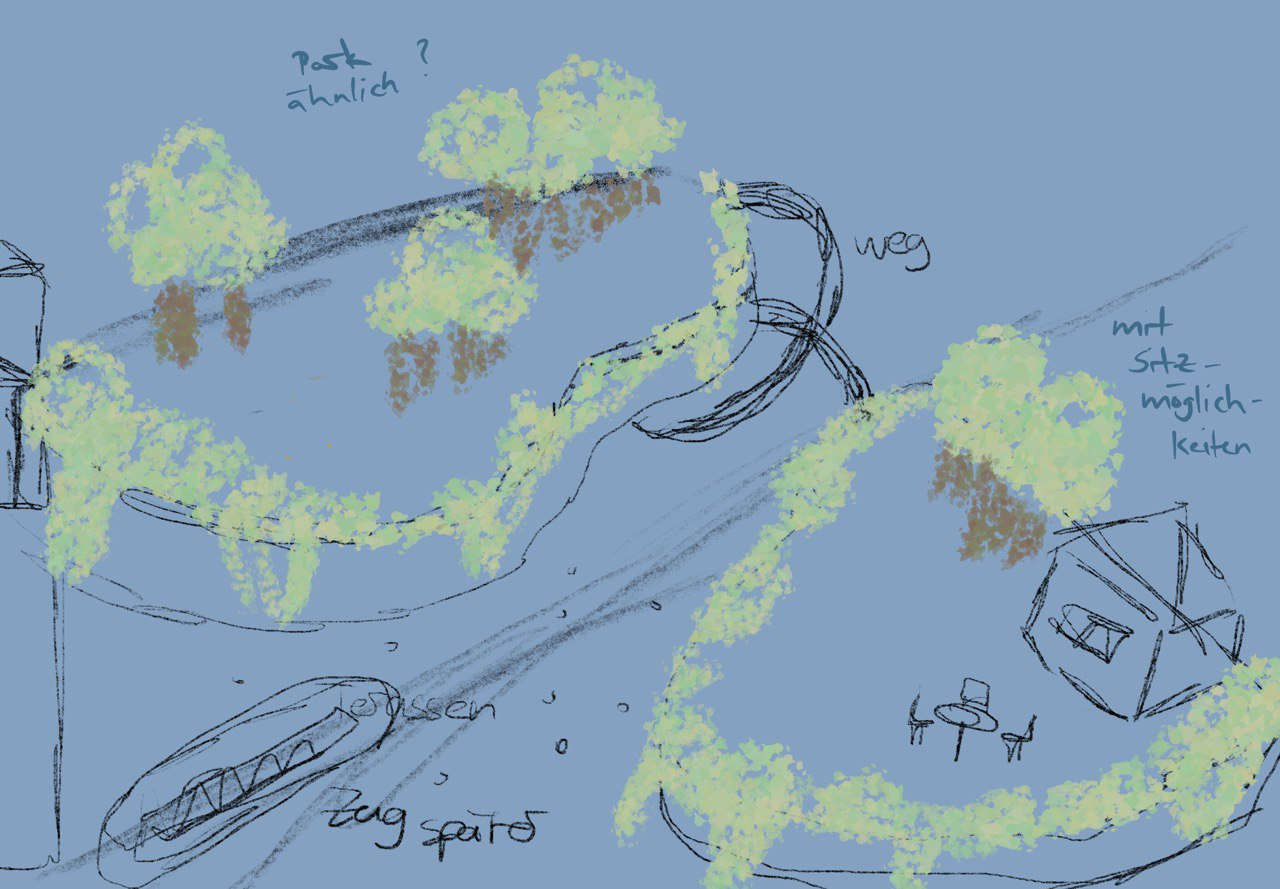
\includegraphics[height=0.3\pageheight,keepaspectratio]{pics/4} 
		\caption{Szene für das MVP}
	\end{subfigure}	
	\caption{Konzeptskizzen für die Szene}
\end{figure}
\par
Speziell auf das MVP ausgerichtet, habe ich die Skizzen vereinfacht und eine gänzlich neue Form in Betracht gezogen, die nach einigen Anpassungen schließlich die finale Gestalt annahm. Im späteren Verlauf war es natürlich auch erforderlich, Texturen für die Modelle zu erstellen. Auf diesen Aspekt werde ich im Implementierungsteil noch einmal eingehen.
\begin{figure}[h]
	\centering
	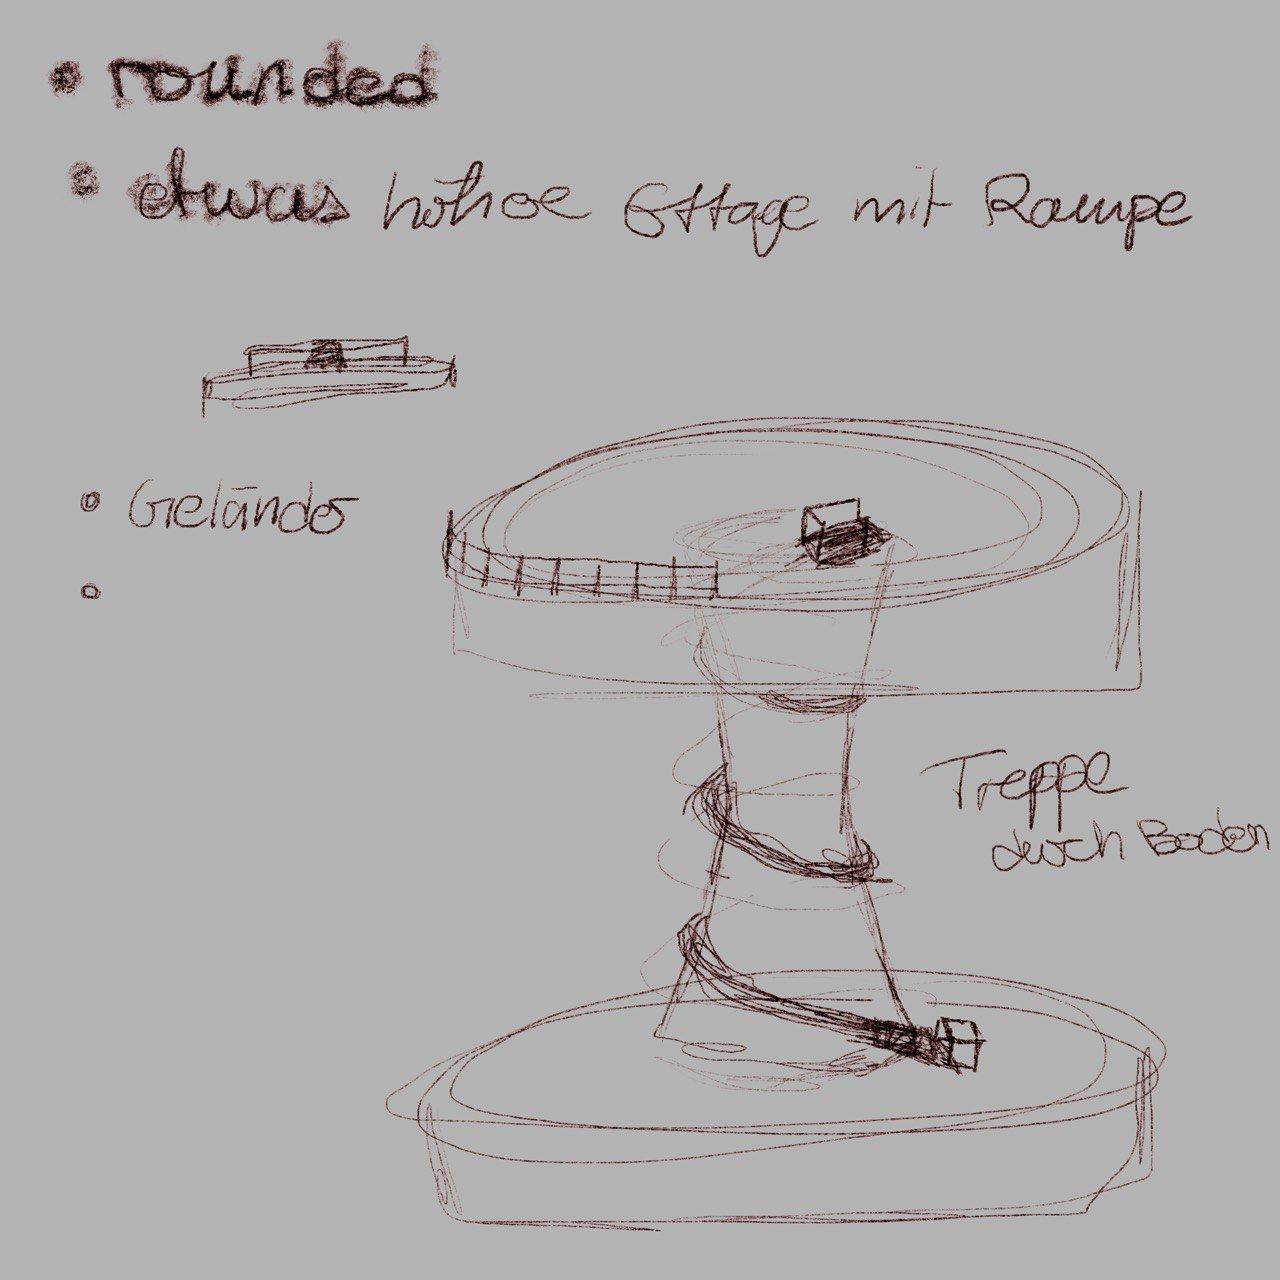
\includegraphics[height=0.3\pageheight,keepaspectratio]{pics/5} 
	\caption{Finaler Entwurf die Szene für das MVP}
\end{figure}
